%% LyX 2.1.4 created this file.  For more info, see http://www.lyx.org/.
%% Do not edit unless you really know what you are doing.
\documentclass[english]{article}
\usepackage[T1]{fontenc}
\usepackage[latin9]{inputenc}
\usepackage{geometry}
\geometry{verbose,tmargin=2cm,bmargin=2cm,lmargin=2cm,rmargin=2cm}
\usepackage{textcomp}
\usepackage{amsmath}
\usepackage{graphicx}
\usepackage{esint}

\makeatletter

%%%%%%%%%%%%%%%%%%%%%%%%%%%%%% LyX specific LaTeX commands.
%% Because html converters don't know tabularnewline
\providecommand{\tabularnewline}{\\}
%% A simple dot to overcome graphicx limitations
\newcommand{\lyxdot}{.}


%%%%%%%%%%%%%%%%%%%%%%%%%%%%%% User specified LaTeX commands.
\usepackage{babel}

\makeatother

\usepackage{babel}
\begin{document}

\title{Parameter studies for REXI}


\author{Martin Schreiber <M.Schreiber@exeter.ac.uk>\\
 et al.}

\maketitle
This documents is on results for the REXI (In this work, we refer
to REXI as described in \cite{Terry:High-order time-parallel approximation of evolution operators}\cite{Schreiber:Understanding_REXI})
and is based on the linear formulation of the SWE only. The main for
creating this document were questions on the dependency of the REXI
parameters $h$ and $M$ on the given scenarios described by the linear
operator $L$ and the initial conditions.

Several benchmarks are executed to evaluate these dependencies of
the REXI parameters on scenarios representative for geophysical flows.

For sake of reproducibility, the benchmarks are given by (benchmark:
{[}directory name{]}).


\section{Benchmark scenario description}


\subsection{Equations}

We analyze the behavior of REXI based on parameter studies of the
linear part 
\[
L(U):=\left(\begin{array}{ccc}
0 & -\eta_{0}\partial_{x} & -\eta_{0}\partial_{y}\\
-g\partial_{x} & 0 & f\\
-g\partial_{y} & -f & 0
\end{array}\right)U
\]
of the SWE (see \cite{Schreiber:Formulations of the shallow-water equations},
note that the sign is inverted) with 
\[
U_{t}=\epsilon L(U)
\]
with
\[
U:=(h,u,v)^{T}.
\]
If not otherwise stated, we set $\epsilon=g=\eta_{0}=f=1$ and $\Omega=[0;1]^{2}$.


\subsection{Abbreviations}

We give a brief overview of the used abbreviations for the parameter
studies:

\begin{tabular}{|c|l|}
\hline 
\textbf{Symbol} & \textbf{Description}\tabularnewline
\hline 
\hline 
$h$ & REXI parameter specifying the sampling accuracy\tabularnewline
\hline 
$M$ & REXI parameter related to the number of poles\tabularnewline
\hline 
$NxN$ & Resolution of simulation domain\tabularnewline
\hline 
$\tau$ & Time step size for REXI\tabularnewline
\hline 
$dt$ & Time step size for REXI (identical to $\tau$ in this work)\tabularnewline
\hline 
$DT$ & Overall simulation time\tabularnewline
\hline 
$nT$ & Number of time steps\tabularnewline
\hline 
$W$ & Parameter related to the number of waves in the initial conditions\tabularnewline
\hline 
\end{tabular}


\subsection{Initial conditions}

\label{sub:initial_conditions}We consider the following initial conditions


\subsubsection{Scenario ``Gaussian'' (Default)}

If not otherwise stated, we use the Gaussian function
\begin{eqnarray*}
\eta(x,y) & := & \eta_{0}+e^{-50(x^{2}+y^{2})}\\
u(x,y) & := & 0\\
v(x,y) & := & 0
\end{eqnarray*}
as initial conditions and use zero values for initial velocity conditions.


\subsubsection{Scenario ``Waves''}

\label{sub:scenario_waves}We also evaluate the following initial
parameter from \cite{Terry:High-order time-parallel approximation of evolution operators}:
\begin{eqnarray*}
h(x,y) & := & sin(6\pi x)cos(4\pi y)-\frac{1}{5}cos(4\pi x)sin(2\pi y)+\eta_{0}\\
u(x,y) & := & cos(6\pi x)cos(4\pi y)-4sin(6\pi x)sin(4\pi y)\\
v(x,y) & := & cos(6\pi x)cos(6\pi y)
\end{eqnarray*}



\subsubsection{Scenario ``Frequencies''}

\label{sub:scenario_frequencies}For testing different frequencies
in the initial conditions, we also introduce additional frequencies
via the parameter $W$ by setting

\begin{eqnarray*}
fx & := & \pi\cdot x\cdot W\\
fy & := & \pi\cdot y\cdot W
\end{eqnarray*}
and use the following initial conditions:

\begin{eqnarray*}
h(x,y) & := & sin(2\,fx)\,cos(2\,fy)-\frac{1}{5}cos(2\,fx)\,sin(4\,fy)+\eta_{0}\\
u(x,y) & := & cos(4\,fx)\,cos(2\,fy)\\
v(x,y) & := & cos(2\,fx)\,cos(4\,fy)
\end{eqnarray*}



\subsection{Discretization in time}

A Runge-Kutta time stepping method of 4-th order is used if appropriate.
E.g. RK4 is not used for REXI, but for the other methods discussed
in the next section.


\subsection{Solvers and their discretization in space}

\label{sub:discretization_in_space}The tests are based on different
implementations in space:


\subsubsection{Used derivatives}

\label{sub:discretization_derivatives_fd_sp}The derivatives in the
linear operator $L$ can be based on
\begin{itemize}
\item (FDderiv) Finite difference methods (e.g. a $[-1,0,1]$ stencil) or
\item (SPderiv) computing the derivative via the spectral basis functions
($\frac{d}{dx}e^{ixj2\pi}$).
\end{itemize}

\subsubsection{Realization of operator}

Derivatives can be expressed either in
\begin{itemize}
\item (Cop) Cartesian space via a stencil computation (expensive in Cartesian
space) or
\item (Sop) Spectral (Fourier) space via a spectral convolution (element-wise
multiplication and hence very cheap in spectral space).
\end{itemize}

\subsubsection{Grid alignment}
\begin{itemize}
\item (A-grid): All conserved quantities are placed at the cell center
\item (C-grid): The potential is placed at the cell center and the velocity
components at the cell edges.\\
Furthermore, computations are based on the vector invariant formulation.
\end{itemize}

\subsubsection{REXI}

There is only one REXI implementation considered, but with different
parameters which are discussed below.


\subsection{REXI}

The REXI approach allows testing different parameters. In this work,
we analyze the accuracy of REXI, based on the parameters $h$ and
$M$, see \cite{Schreiber:Understanding_REXI} for their description.
The approximation is then given by a sum over a system of independent
systems of equations to be solved:

\begin{equation}
e^{\tau L}\approx\sum_{n=0}^{N}\frac{\gamma_{n}^{Re}}{\tau L+\alpha_{n}}\label{eq:rexi_approx}
\end{equation}
We denote the result $U'(\tau)$ of the REXI approach by
\[
U'(\tau):=REXI(U(0),\tau,h,M)
\]
with $U$ the solution at $t=0$, the parameter $\tau$ the size of
the large time step, $h$ the sampling interval size and $M$ related
to the number of poles $K+M+1$ used to compute REXI to $L$.


\subsection{Error norm}

We use the RMS error norm 
\[
RMS(f):=\sqrt{\frac{\sum_{\vec{x}}\left(f_{\vec{x}}-\tilde{f}_{\vec{x}}\right)^{2}}{\prod_{i}\vec{N}_{i}}}
\]
based on a discrete computed solution $f_{\vec{x}}$ for the points
given by $\vec{x}_{i}\in\{0,1,...,\vec{N}_{i}\}$, the reference solution
given by $\tilde{f}(\vec{x})$ and with each component in $\vec{N}$
giving the resolution. In this work we only compare the RMS to the
height $\eta$.


\section{Analytical benchmark results}


\subsection{Study for REXI parameters $h$ and $M$}

(benchmark folder: 2015\_09\_04\_search\_h\_M)

We first search for an optimal choice of $h$ and $M$ values. $h$
is a value which only relates to the accuracy of the REXI approximation
and $M$ relates to the accuracy, as well as to the computational
workload which has to be invested for the REXI approach. We execute
the simulation for an overall simulation time of $DT:=1$ second and
use a time step size for REXI of $dt:=0.1$. Hence, 10 time steps
with REXI are executed. The results are given based on the computation
of the RMS error on the height $\eta$.


\subsubsection{Different resolutions}

We first conduct a parameter study for different resolutions\\


\begin{tabular}{cc}
\includegraphics[width=0.45\textwidth]{results_plots/2015_09_04_search_h_M/output_n16_eps1_dt0\lyxdot 1} & \includegraphics[width=0.45\textwidth]{results_plots/2015_09_04_search_h_M/output_n32_eps1_dt0\lyxdot 1}\tabularnewline
\includegraphics[width=0.45\textwidth]{results_plots/2015_09_04_search_h_M/output_n64_eps1_dt0\lyxdot 1} & \includegraphics[width=0.45\textwidth]{results_plots/2015_09_04_search_h_M/output_n128_eps1_dt0\lyxdot 1}\tabularnewline
\end{tabular}

We can observe a (blue-colored) triangle with high-accurate solutions
of $O(10^{-6})$. This optimal triangle area for a given numerical
accuracy $e$ can be described by
\[
A_{(M,h)}:=\{(M,h)|Mh>C(e),\,h<0.5\}
\]
with $C:=1024$ for an accuracy $\approx10^{-7}$.

We account for the diagonal edge at $Mh=const.$ by $h$ specifying
the sampling interval and $M$ the sampling nodes. If a smaller value
of $h$ results in an oversampling of the frequency, more poles $M$
have to be used to accurately cover the approximation of the solution.
Since we should try to minimize $M$ as far as possible, we can determine
a particular best-investment for $M$ at the left lower corner of
the triangle area by choosing $h\in[0.125,\,0.25]$.

We define such an optimal choice of $h$ and $M$ as the sweetspot
for a given numeric solution $U'(t+\tau,h,M):=REXI(U(t),\tau,h,M)$
and a given numerical error threshold$e$. We then search for parameters
$(M,h)$ which keep the error below a certain error threshold~$e$
and minimize the number of poles directly related to $M$. Then, this
sweetspot is given by 
\[
S(h,M):=min_{M}min_{h}\left(rms\left(U'(t+\tau,h,M)-U(t\tau)\right)<e\right)
\]
for the optimal choice of the parameters $(h,M)$.


\subsubsection{Dependency of $h$ and $M$ on different resolutions $N$}

Next, we test if both parameter changes for different resolutions
(see above) and we can observe, that $h$ can be fixed and we use
$h:=0.2$ if not otherwise stated.

For these conducted benchmarks, a change in resolution did not significantly
change the results for selected parameters $h$ and $M$. Here, we
like to mention, that this independency depends on the solver for
$(L+\alpha)^{-1}$ and refer to Section \ref{sub:finite_differences_for_solver}.


\subsubsection{Summary}

\begin{tabular}{|r|l|}
\hline 
\textbf{REXI parameter} & \textbf{Observation}\tabularnewline
\hline 
\hline 
$h$ & Optimum given at $h:=0.2$\tabularnewline
\hline 
$M$ & Independent to the resolution\tabularnewline
\hline 
\end{tabular}

Given a desired numerical accuracy $e$ and with $h:=0.2$ assumed
to be constant, the optimal parameters $M$ is given by
\begin{equation}
M:=\frac{C(e)}{h}.\label{eq:summary_m_c_h}
\end{equation}



\subsection{Testing for different $\epsilon$}

(benchmark folder: 2015\_08\_30\_search\_epsilons, 2015\_09\_03\_search\_epsilons,
2015\_09\_03\_search\_epsilons\_b)

The REXI approach should hold for all the possible regimes of atmospheric
constellations. Therefore, we generalize our formulation with $\epsilon$
\[
U_{t}=\epsilon L(U)
\]
which we realize by setting $g=\eta_{0}=f=\epsilon$ in our simulations.


\subsubsection{Studies for $\epsilon:=\{1,\,0.1,\,0.01\}$}

We fix our test resolution to $64^{2}$ for this evaluation and show
plots for $\epsilon:=\{1,\,0.1,\,0.01\}$:

\begin{tabular}{cc}
\includegraphics[width=0.45\textwidth]{results_plots/2015_08_30_search_epsilons/output_64_eps0\lyxdot 01} & \includegraphics[width=0.45\textwidth]{results_plots/2015_08_30_search_epsilons/output_64_eps0\lyxdot 10}\tabularnewline
\includegraphics[width=0.45\textwidth]{results_plots/2015_08_30_search_epsilons/output_64_eps1\lyxdot 00} & \includegraphics[width=0.45\textwidth]{results_plots/2015_08_30_search_epsilons/output_128_eps0\lyxdot 01}\tabularnewline
\end{tabular}

For a decreasing $\epsilon$, we can see that the previously clear
optimal parameters for $(h,M)$ are now getting more diffusive. To
see if the parameters $(h,M)$ depend on the resolution, we added
a plot for benchmarks with the resolution $128^{2}$ and $\epsilon:=0.01$,
see right bottom in the figures above. We can see, that the parameters
of the REXI approach are again independent to the resolution for this
scenario.


\subsubsection{Studies for $\epsilon:=\{10,100\}$}

Since the borders got more diffusive for $\epsilon\ll1$, we expect
a sharp border for $\epsilon\gg1$ which we evaluate next for sake
of curiosity:

\begin{tabular}{cc}
\includegraphics[width=0.45\textwidth]{results_plots/2015_08_30_search_epsilons/output_64_eps10\lyxdot 00} & \includegraphics[width=0.45\textwidth]{results_plots/2015_08_30_search_epsilons/output_64_eps100\lyxdot 00}\tabularnewline
\end{tabular}

However, we don't see an increase in diffusiveness. But we can observe,
that the solution area $A_{(M,h)}$ is shifted to the right side.
Hence, for larger $\epsilon$ values (this increases the stiffness
of the problem), we also have to increase $M$. We observe again,
that the solution area $A_{(M,h)}$ still seems to be independent
to the choice of $h\approx0.2$.


\subsubsection{Dependency of $M$ to $\epsilon$}

\label{sub:dep_of_M_to_eps}To determine the dependency of $M$ to
$\epsilon$, we finally executed a parameter study by setting $h:=0.2$
and with variables $\epsilon$ and $M$. Here, we keep the simulated
time limited to $dT:=1$ and use a REXI timestep size of $dt:=0.1$.\\


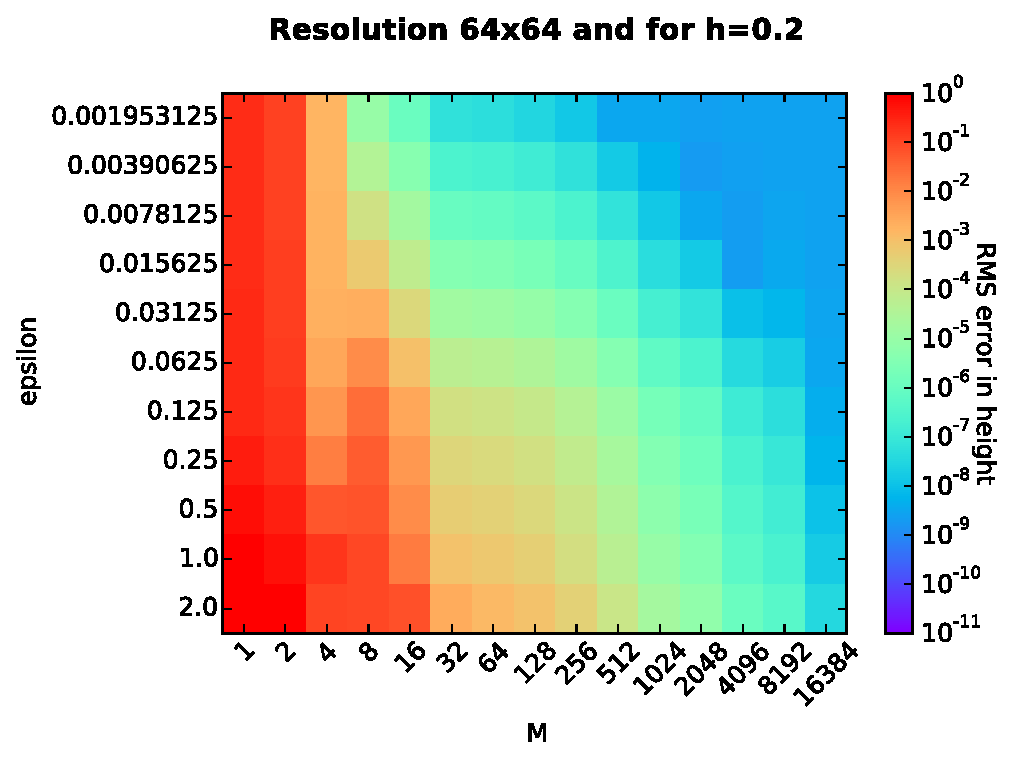
\includegraphics[width=0.45\textwidth]{results_plots/2015_09_03_search_epsilons_b/output_n64}

We can see a linear dependency of $M$ to $\epsilon$ in the range
of$\epsilon\in[0.01;1]$.


\subsubsection{Summary}

Regarding the results from Section \ref{sub:dep_of_M_to_eps}, the
REXI parameter $M$ is proportional to $\epsilon$: The larger the
$\epsilon$, the more poles have to be used for an approximation of
sufficient accuracy. In combination with Eq. \eqref{eq:summary_m_c_h},
we can extend the formula for automatically determining $M$ to 
\begin{equation}
M:=\frac{C(e)\epsilon}{h}.\label{eq:summary_m_c_h_eps}
\end{equation}


This dependency to $\epsilon$ gets more obvious with a straight-forward
EV decomposition of $L$:
\[
U(t):=e^{\epsilon tL}U(0):=\Sigma\Lambda\Sigma^{-1}U(0)=\Sigma\left[\begin{array}{ccc}
e^{\epsilon t\lambda_{0}}\\
\\
 &  & e^{\epsilon t\lambda_{n}}
\end{array}\right]\Sigma^{-1}U(0)=\Sigma e^{\epsilon t\Lambda}\Sigma^{-1}U(0)
\]
with imaginary eigenvalues $\lambda_{i}$ as the diagonal in $\Lambda$.
Therefore, larger values of $\epsilon$ also lead to faster oscillations
in the solution. Therefore, more poles have to be invested to capture
these frequencies which is specified by $M$.


\subsection{Study for REXI parameter $M$ and resolution $NxN$}

We start by evaluating the dependency of the REXI parameter $M$ to
the resolution $NxN$ by a single time step. We again set $h:=0.2$
for these benchmarks and evaluate the dependency with the initial
conditions described in Section \eqref{sub:initial_conditions}.


\subsubsection{Single time step}

(benchmark: 2015\_09\_04\_increasing\_dt\_single\_timestep\_s1, 2015\_09\_04\_increasing\_dt\_single\_timestep\_s5)

The first tests are performed with a single time step and varying
time step size.

We first have a look on the results for the Gaussian initial conditions:

\begin{tabular}{cc}
\includegraphics[width=0.45\textwidth]{results_plots/2015_09_04_increasing_dt_single_timestep_s1/output_n32_eps1_h0\lyxdot 2} & \includegraphics[width=0.45\textwidth]{results_plots/2015_09_04_increasing_dt_single_timestep_s1/output_n64_eps1_h0\lyxdot 2}\tabularnewline
\end{tabular}

We can observe, that there is indeed a dependency on the used resolution.
However, this can be induced by using zero-valued velocity components
as initial conditions. Therefore, we further evaluate this with initial
conditions with non-zero velocities based on the wave initial conditions
(see Sec. \ref{sub:scenario_waves}):

\begin{tabular}{cc}
\includegraphics[width=0.45\textwidth]{results_plots/2015_09_04_increasing_dt_single_timestep_s5/output_n32_eps1_h0\lyxdot 2} & \includegraphics[width=0.45\textwidth]{results_plots/2015_09_04_increasing_dt_single_timestep_s5/output_n64_eps1_h0\lyxdot 2}\tabularnewline
\end{tabular}

Here, we can observe that the accuracy of the solution again is independent
to the resolution. An increasing time step size $dt$ shows a linear
dependency of $M$ on $dt$.


\subsubsection{Multiple time steps}

(benchmark: 2015\_09\_04\_increasing\_dt\_10\_timesteps\_s1, 2015\_09\_04\_increasing\_dt\_10\_timesteps\_s5)

Next, we analyze the accuracy over multiple time steps with the Gaussian
and Waves as initial conditions:

\begin{tabular}{cc}
\includegraphics[width=0.45\textwidth]{results_plots/2015_09_04_increasing_dt_10_timesteps_s1/output_n32_eps1_h0\lyxdot 2} & \includegraphics[width=0.45\textwidth]{results_plots/2015_09_04_increasing_dt_10_timesteps_s1/output_n64_eps1_h0\lyxdot 2}\tabularnewline
\includegraphics[width=0.45\textwidth]{results_plots/2015_09_04_increasing_dt_10_timesteps_s5/output_n32_eps1_h0\lyxdot 2} & \includegraphics[width=0.45\textwidth]{results_plots/2015_09_04_increasing_dt_10_timesteps_s5/output_n64_eps1_h0\lyxdot 2}\tabularnewline
\end{tabular}

We can again observe, that the results show an independence to the
resolution. Again, an increasing time step size $dt$ results in a
linear increase of $M$.


\subsubsection{Different time step sizes over varying resolution $N$ and $M$}

(benchmark: 2015\_09\_04\_study\_N\_M\_small\_ts)

The independence to the resolution can be caused by the large time
step size dominating the error. To check that the error in time is
not dominating (which would explain the independence of $M$ to the
resolution), we further analyze the error with very small time step
sizes $dt$, varying $M$ and varying resolution $N$:

\begin{tabular}{cc}
\includegraphics[width=0.45\textwidth]{results_plots/2015_09_04_study_N_M_small_ts/output_eps1_dt0\lyxdot 01_DT0\lyxdot 01} & \includegraphics[width=0.45\textwidth]{results_plots/2015_09_04_study_N_M_small_ts/output_eps1_dt0\lyxdot 001_DT0\lyxdot 01}\tabularnewline
\includegraphics[width=0.45\textwidth]{results_plots/2015_09_04_study_N_M_small_ts/output_eps1_dt0\lyxdot 0001_DT0\lyxdot 01} & \includegraphics[width=0.45\textwidth]{results_plots/2015_09_04_study_N_M_small_ts/output_eps1_dt1e-05_DT0\lyxdot 01}\tabularnewline
\end{tabular}\\
\\
For these small time step sizes, we can observe, that the change in
resolution still does not result in any change regarding the parameter
$M$ depending on the resolution $N$.


\subsubsection{Conclusion}

An increasing time step size $dt$ requires a linear increase of $M$.
Therefore, we extend Equation \eqref{eq:summary_m_c_h_eps} with $dt$.

\begin{equation}
M:=\frac{dt\,C(e)}{h\epsilon}.\label{eq:summary_m_dt_c_h_eps}
\end{equation}



\subsection{Finite-difference-based solution for $(\tau L-\alpha)^{-1}$}

\label{sub:finite_differences_for_solver}Since we use a spectral
solver to solve for $(\tau L-\alpha)^{-1}$, this can be the reason
of $M$ being independent to the resolution $M$. Therefore, we run
tests with an alternative solver in spectral space (to avoid implementing
time-consuming alternative solvers): One which does not setup the
derivative operator in spectral space (e.g. based on $\frac{\partial}{\partial x}e^{ixk}\tilde{u}(k)=ike^{ixk}\tilde{u}(k)$),
but one which is based on a finite difference operator (e.g. $\frac{\partial}{\partial x}u(x)\approx\frac{u_{x+h}-u_{x-h}}{2h}$)
specified in Cartesian space (see also Section \ref{sub:discretization_derivatives_fd_sp}),
but applied as a folding operation in Fourier space.

Note, that despite we are using the Fourier space to solve this, the
results are representative for the solution which would be computed
with alternative solvers such as based on an LU decomposition or iterative
solvers.


\subsubsection{Studies for varying $h$ and $M$}

(benchmark: 2015\_09\_07\_search\_h\_M\_finite\_differences)\\


\begin{tabular}{cc}
\includegraphics[width=0.45\textwidth]{results_plots/2015_09_07_search_h_M_finite_differences/output_n16_eps1_dt0\lyxdot 1} & \includegraphics[width=0.45\textwidth]{results_plots/2015_09_07_search_h_M_finite_differences/output_n32_eps1_dt0\lyxdot 1}\tabularnewline
\includegraphics[width=0.45\textwidth]{results_plots/2015_09_07_search_h_M_finite_differences/output_n64_eps1_dt0\lyxdot 1} & \includegraphics[width=0.45\textwidth]{results_plots/2015_09_07_search_h_M_finite_differences/output_n128_eps1_dt0\lyxdot 1}\tabularnewline
\end{tabular}

For the $16^{2}$ resolution, we like to mention that the initial
conditions are barely captured by this resolution.

Compared to computing $(L+\alpha)^{-1}$ with spectral methods, 
\begin{itemize}
\item Accuracy: We observe now a significantly reduced accuracy
\item Optimal solution area: We can observe a similar ``triangular''-shaped
solution area. However, the $h$ values can be larger.
\item Dependency of $M$ to the resolution $N$.\\
For the larger resolution $128^{2}$, there seems to be a dependency
of $M$ to the resolution $N$, however there's not a clear significance
given
\end{itemize}

\subsubsection{Studies for varying $h$ and $M$: refined $h$ \& $N$}

(benchmark: 2015\_09\_07\_search\_h\_M\_finite\_differences\_2)

Based on the previous results, we continue with additional parameter
studies, but with $h$ refined around the optimum interval $\{0.1,0.2,...,2.0\}$
and with larger resolutions to determine if there's a dependency of
$M$ to the resolution.

\textbf{Note the different scaling for the coloring which we did for
sake of clarity!}

\begin{tabular}{cc}
\includegraphics[width=0.45\textwidth]{results_plots/2015_09_07_search_h_M_finite_differences_2/output_n16_eps1_dt0\lyxdot 1} & \includegraphics[width=0.45\textwidth]{results_plots/2015_09_07_search_h_M_finite_differences_2/output_n32_eps1_dt0\lyxdot 1}\tabularnewline
\includegraphics[width=0.45\textwidth]{results_plots/2015_09_07_search_h_M_finite_differences_2/output_n64_eps1_dt0\lyxdot 1} & \includegraphics[width=0.45\textwidth]{results_plots/2015_09_07_search_h_M_finite_differences_2/output_n128_eps1_dt0\lyxdot 1}\tabularnewline
\includegraphics[width=0.45\textwidth]{results_plots/2015_09_07_search_h_M_finite_differences_2/output_n256_eps1_dt0\lyxdot 1} & \includegraphics[width=0.45\textwidth]{results_plots/2015_09_07_search_h_M_finite_differences_2/output_n512_eps1_dt0\lyxdot 1}\tabularnewline
\end{tabular}

Here, we can observe indeed the requirement of $M$ to be increased
if also a decrease in error should be obtained. There also seems to
be a linear dependence of $M$ to the resolution $N$.


\subsubsection{Conclusion}

When using a finite-difference solver or any other solvers based on
1st order accurate approximations of the solution (e.g. finite-element
with 1st order basis functions), this requires a dependency of $M$
on the resolution $N$. We use the subindex to differentiate this
determination of $M$ to the one for a spectral solver.

\begin{equation}
M_{FD}:=\frac{dt\,C_{FD}(e)\,N}{h\epsilon}.\label{eq:summary_m_dt_c_h_eps-1}
\end{equation}
We should emphasize, that here the desired accuracy specified by $e$
may be not achieved due to space-discretization errors. Finally we
mention that the $C(e)$ already included the accuracy, hence this
formula for determining $M$ can be rewritten by making $C$ dependent
on $N$.


\subsection{Dependency of $M$ on number of waves $W$ in initial conditions}

The REXI approach approximates the linear operator $L$ acting on
initial conditions. Hence, this approximation has to be able to capture
all waves in the initial condition. Therefore, we next evaluate the
possible dependency $M$ on the number of frequencies in the initial
condition (see Section \ref{sub:scenario_frequencies}). We briefly
like to mention, that we skipped showing the resolutions $32\text{\texttwosuperior}$
and $64\text{\texttwosuperior}$ here, since all frequencies of the
initial conditions cannot be captured by the grid resolution. We evaluated
these studies with $h:=0.8$. Smaller values of $h$ only resulted
in a decrease of accuracy for a fixed $M$.


\subsubsection{Spectral REXI:}

The simulation is executed over $DT:=50$ with $dt:=5$.\\
\begin{tabular}{cc}
\includegraphics[width=0.45\textwidth]{results_plots/2015_09_25_search_M_vs_waves/summary_rexi_spec_par_h08_error_n0128} & \includegraphics[width=0.45\textwidth]{results_plots/2015_09_25_search_M_vs_waves/summary_rexi_spec_par_h08_error_n0256}\tabularnewline
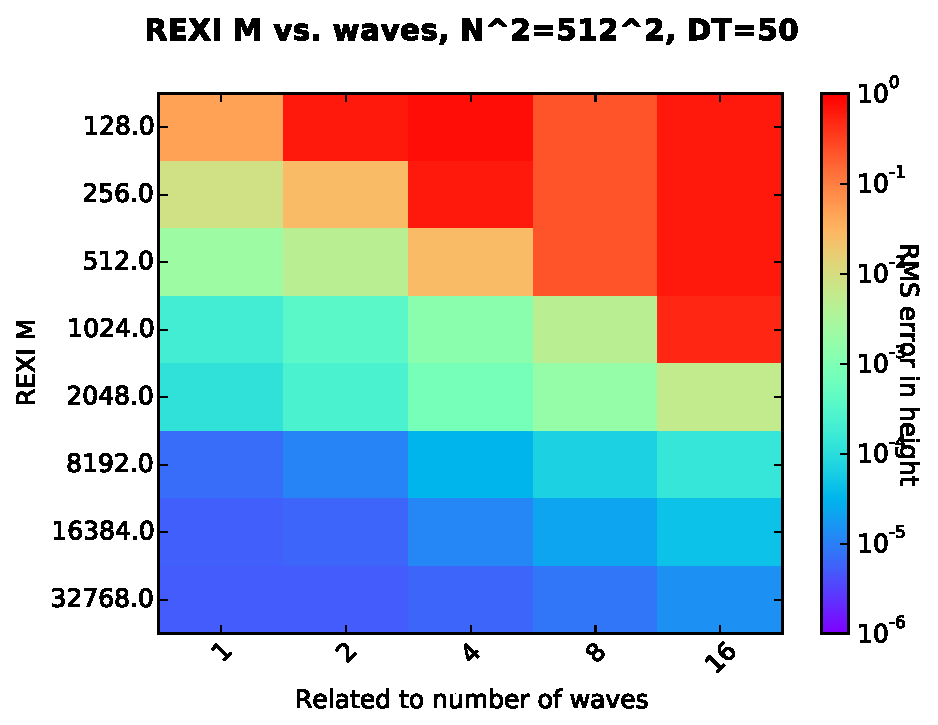
\includegraphics[width=0.45\textwidth]{results_plots/2015_09_25_search_M_vs_waves/summary_rexi_spec_par_h08_error_n0512} & \tabularnewline
\end{tabular}

We can observe, that for an increase of frequencies in the initial
conditions (related to $W$), also an increase of the number of poles
$M$ for the REXI approximation is required in spectral space. The
apparent independence of $M$ to the resolution was already discussed
in a previous Section which we expect to be dependent by using finite
differences which we evaluate next.


\subsubsection{Finite-difference REXI}

We evaluate the accuracy and dependence of $M$ on the resolution
$N$ and the number of waves $W$. \\
\begin{tabular}{cc}
\includegraphics[width=0.45\textwidth]{results_plots/2015_09_25_search_M_vs_waves/summary_rexi_fd_par_h08_error_n0128} & \includegraphics[width=0.45\textwidth]{results_plots/2015_09_25_search_M_vs_waves/summary_rexi_fd_par_h08_error_n0256}\tabularnewline
\includegraphics[width=0.45\textwidth]{results_plots/2015_09_25_search_M_vs_waves/summary_rexi_fd_par_h08_error_n0512} & \tabularnewline
\end{tabular}

The accuracy of these simulations are significantly worse than the
ones with the spectral solver. We like to mention, that we executed
these studies over a very large time step size of $DT:=50$ which
leads to these high inaccuracies. We can observe, that in these benchmarks,
the parameter $M$ also depends on the number of waves.


\subsubsection{Conclusion}

The number of poles for the REXI approximation depends on the frequencies
in the solution. Since these frequencies are in general not known
for arbitrary simulation states (assuming that a Fourier transformation
is not feasible), the parameter \textbf{$M$ has to be set to capture
also the highest frequencies $W$.}


\section{Comparison with Terry's paper}

\textbf{{[}TODO{]} These results match with Terrys paper.}


\section{Performance benchmarks and comparison to standard time stepping schemes}

Here, we compare the REXI approach with several other possible discretizations,
see Sec. \ref{sub:discretization_in_space}.


\subsection{Performance studies for time stepping methods}

(benchmark: 2015\_09\_16\_performance\_and\_scalability\_snb)

We executed performance studies on a 16-core Intel Sandybridge system
(2 sockets, each socket has 8 cores) to compare the overall computation
time of several discretization methods with the REXI approach in both
accuracy and time to solution. For initial conditions, we used the
Gaussian distribution which generates frequencies over the entire
band in Fourier space.

The initial conditions are given by the Gaussian distribution (see
Sec. \ref{sub:initial_conditions}). For the non-REXI approaches,
we use a $CFL:=0.3$ and RK4 time stepping method. For the approximated
solution with REXI, a time step size of $dt:=5$ is used. All simulations
were executed over $DT:=50$ simulation seconds.


\subsection{Error}

We first evaluate the errors for different time stepping methods,
including REXI to compare the performance of similar results.

The following plot shows the results for the finite difference space
discretization:\\


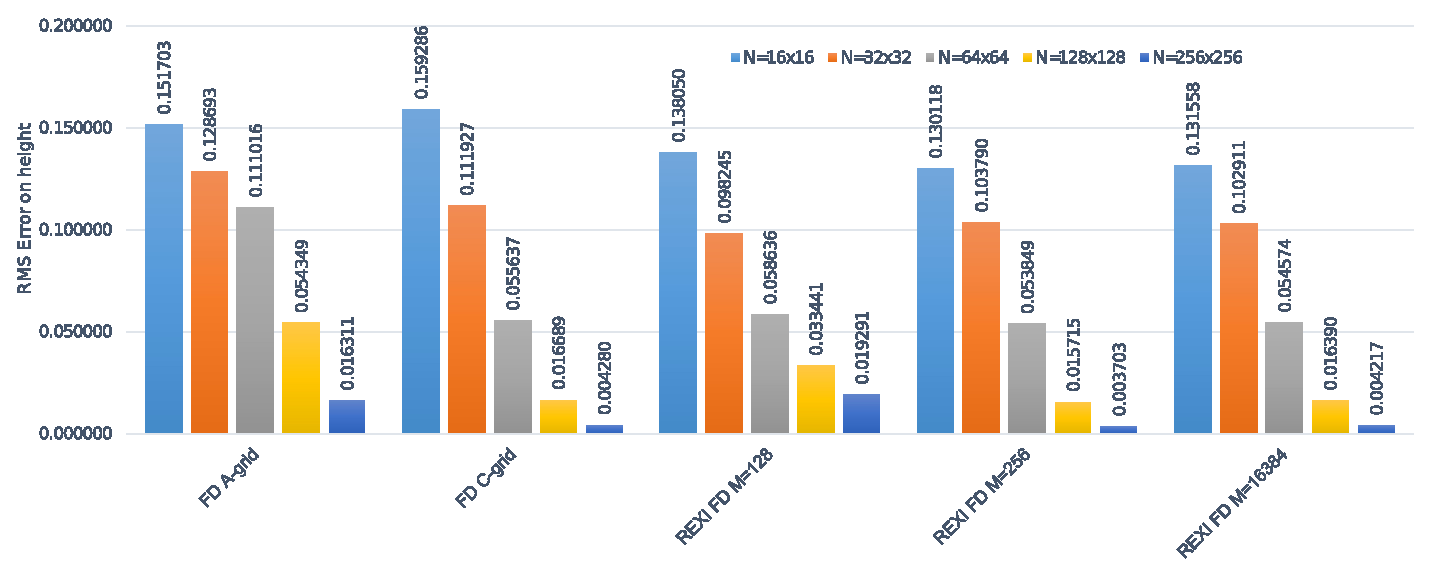
\includegraphics[width=0.95\textwidth]{results_plots/2015_09_16_performance_and_scalability_snb/summary_error_fd}\\


We can observe, that error with the REXI approach and with M=256 poles
are competitive to the finite-difference results.

The next plot shows the accuracy for spectral discretization in space:\\


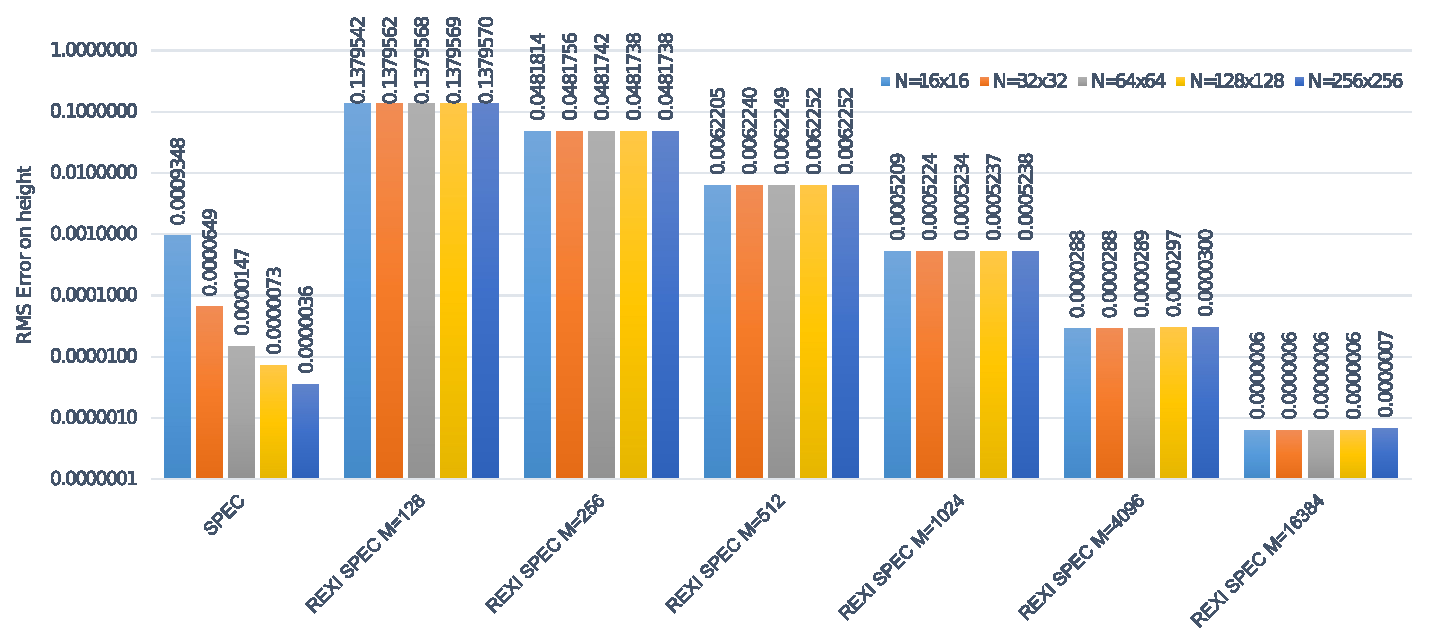
\includegraphics[width=0.95\textwidth]{results_plots/2015_09_16_performance_and_scalability_snb/summary_error_spec}\\


As we can see, only with about $M:=16384$, the REXI approximation
is competitive to the standard spectral method.


\subsection{Parallel performance}

Regarding the parallelization, We tested two different parallelization
concepts for the REXI method:
\begin{itemize}
\item REXI standard: The first one is the default one which parallelizes
over the different solvers
\item REXI PARSUM: The second one uses a parallelization over the sum and
computes each term in the sum using only a single core.
\end{itemize}
We use a resolution of $256^{2}$ for these performance studies.

For sake of reproducibility, we like to mention that we only discuss
the results in this section based on memory allocator version 2 (in
SWEET development) which resulted in the best results. This is a NUMA-aware
memory allocator, avoids allocations on the heap and strongly improves
the performance, hence allows a fair comparison of the computational
amount. A solver in spectral space is used for solving the Helmholtz
equation.


\subsubsection{Finite-differences}

We first have a look on the performance results for the finite difference
method.\\


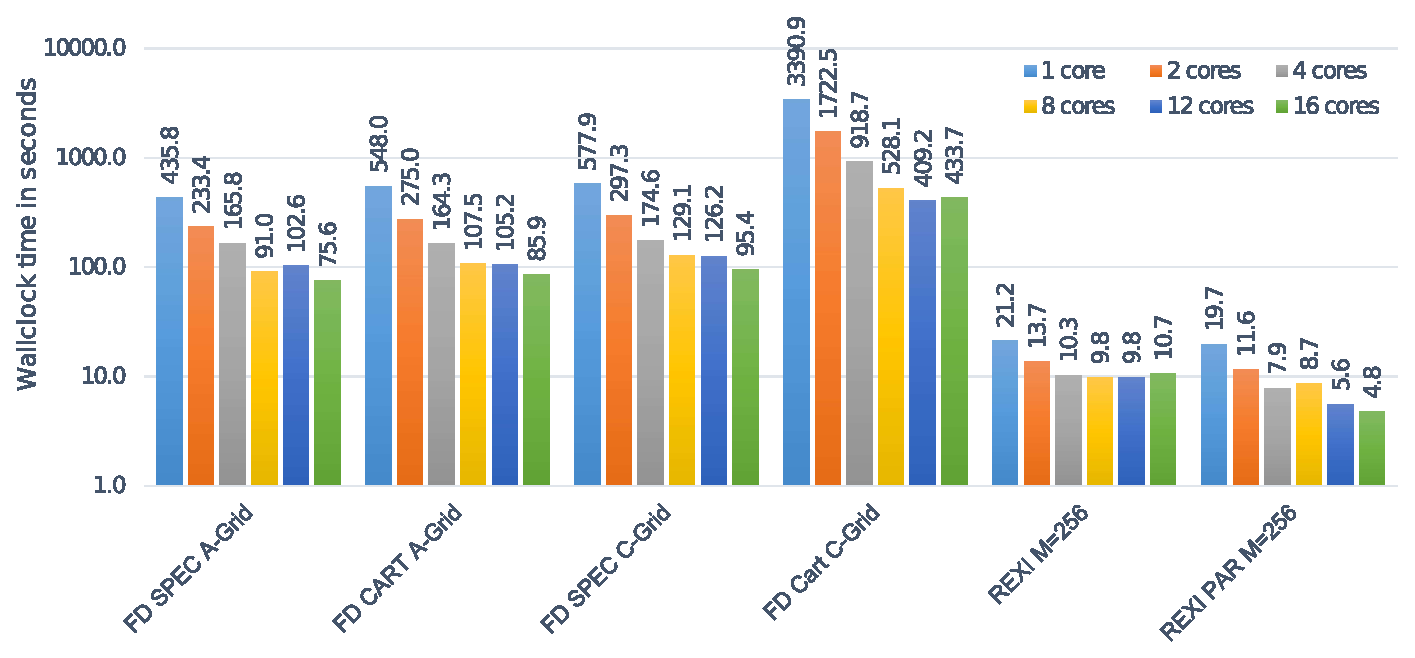
\includegraphics[width=0.95\textwidth]{results_plots/2015_09_16_performance_and_scalability_snb/summary_time_fd}\\


The axis for the wallclock time is in log scale. Comparing the REXI
approach M=256 poles which obtains the same error bounds, we can observe
speedups of $(7.08,\,8.04,\,8.93,\,40.62)$ compared to the standard
time stepping methods from left to right in the performance results,
respectively. We like to mention, that the FD mehtod on the C-grid
was not optimized. Therefore, we consider $8.93$ as a realistic speedup.

Using a parallelization in space, we see a stagnating reduction in
computation time in the 5 left-most groups of performance studies.
With the REXI also a parallelization over the sum itself instead of
a parallelization in space over the term in each sum is possible and
denoted in the performance study above with ``REXI PAR''. In contrast
to the parallelization in space with its scalability limitation already
reached (see REXI M=256) results, we can observe that there is still
an increase in speedup of $1.81$ by doubling the cores from 8 to
16 cores. Comparing both parallelization strategies, the REXI PAR
implementation results in a speedup of $2.23$.

To summarize, we achieve a speedup of $19.88$ for problem sizes for
which a speedup was not achievable with conventional parallelization-in-time
methods.


\subsubsection{Spectral space}

Next, we evaluate possible speedup effects based on a spectral method
used for the standard time stepping with RK4 with a parallelization-in-space:\\


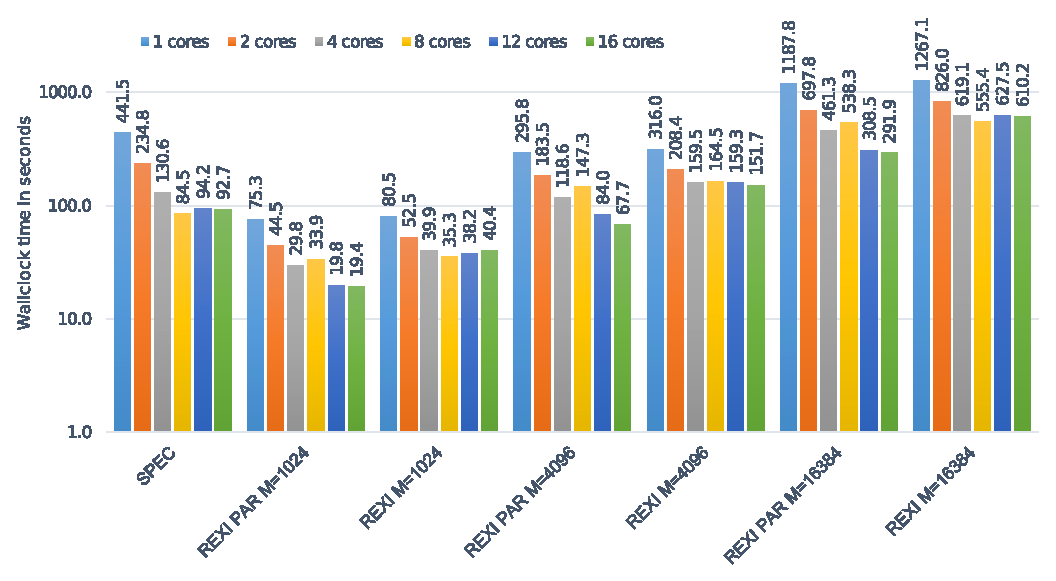
\includegraphics[width=0.95\textwidth]{results_plots/2015_09_16_performance_and_scalability_snb/summary_time_spec}\\


Similar to the finite-difference method, we can observe a stagnation
in the speedup for the parallelization-in-space. With the REXI approach,
we would need $M:=16384$ poles to be competitive to the standard
time stepping solver. Comparing the wallclock time with the best REXI
PAR solver results in a speeddown of $3.15$. We account for that
by the super-convergence of the spectral solvers. However, as an outlook
we should mention that the scalability of the REXI PAR implementation
is not yet reached hence allows using even more cores.


\section{Summary}

{[}TODO{]}


\section{Reproducibility}

There are many variants of implementations possible. To assure a reproducibility
of the presented results, we refer to the SWEET development with which
we generated these results.


\section{Discussion of possible alternative approaches}


\subsection{Eigenvector decomposition in spectral space}

Since the analytical solution is directly given by an Eigenvalue decomposition
in spectral space, this could be an appropriate alternative to using
the REXI approach. This is true for the f-plane. Let's analyze this
property with the $\beta$-plane. Here, the $f$ value is not constant
over the plane, but varies depending on the $y$-coordinate:
\[
f(y):=f_{0}+\beta y
\]


We can now have a look at the spectral formulation of the $L(U)$
operator

\[
-L(U):=\left(\begin{array}{ccc}
0 & \eta_{0}\partial_{x} & \eta_{0}\partial_{y}\\
g\partial_{x} & 0 & -f(y)\\
g\partial_{y} & f(y) & 0
\end{array}\right)U
\]
with $U(\vec{x})$ given by its spectral superposition

\[
U(\vec{x}):=\int_{\vec{k}}\tilde{U}(\vec{k})e^{i\vec{k}\vec{x}}
\]
and $f(\vec{x})$ given by
\[
f(\vec{x}):=\int_{\vec{k}}\tilde{f}(\vec{k})e^{i\vec{k}\vec{x}}.
\]
We were able to compute the solution to $L(U)$ directly in spectral
space with the EV decomposition, since we were able to factor out
the spectral basis functions. An example is given here for the term
$\eta_{0}\partial_{x}$: 
\[
\left(\eta_{0}\partial_{x}\right)\int_{\vec{k}}\tilde{U}(\vec{k})e^{i\vec{k}\vec{x}}=\int_{\vec{k}}\tilde{U}(\vec{k})\eta_{0}\partial_{x}e^{i\vec{k}\vec{x}}=\int_{\vec{k}}\tilde{U}(\vec{k})\eta_{0}i\vec{k}e^{i\vec{k}\vec{x}}=\int_{\vec{k}}\tilde{U}(\vec{k})\left(\eta_{0}i\vec{k}e^{i\vec{k}\vec{x}}\right)
\]
In combination with a Ritz-Galerkin approach and using the orthogonality
of the basis functions, this allows a wave-wise Eigenvalue decomposition.
However for the $f(x)$ term, we are not able to factor out the basis
function and apply the previously mentioned method
\[
\left(f(y)\right)\int_{\vec{k}}\tilde{U}(\vec{k})e^{i\vec{k}\vec{x}}=\int_{\vec{k}}f(\vec{k})e^{i\vec{k}\vec{x}}\int_{\vec{k}}\tilde{U}(\vec{k})e^{i\vec{k}\vec{x}}
\]
which results in a non-linearity. Hence, we are not able to factor
out the spectral basis functions and the approach is not applicable
to the $\beta$-plane anymore.
\begin{thebibliography}{1}
\bibitem{Schreiber:Formulations of the shallow-water equations}Formulations
of the shallow-water equations, M. Schreiber, P. Peixoto

\bibitem{Terry:High-order time-parallel approximation of evolution operators}High-order
time-parallel approximation of evolution operators, T. Haut et al.

\bibitem{Schreiber:Understanding_REXI}Understanding the Rational
Approximation of the Exponential Integrator (REXI), Schreiber M.,
Peixoto P.

\bibitem{Schreiber:SWEET_software}SWEET software development, http://www.martin-schreiber.info/sweet/
, Schreiber M.\end{thebibliography}

\end{document}
